\section{Stacked User Modeling}
\label{sec:usermetamodeling}

How can we perform adaptive method aggregation?
Let us first define a few terms.
We defined \emph{meta modeling} as using one modeling method to adapt other modeling methods.
\emph{User Meta Modeling} would then mean adapting user modeling methods with another user modeling method.
More specifically, we define \emph{stacked user modeling} (SUM) as adapting a set of many user modeling method
with a set of secondary, higher-level modeling methods.
Formally, a system for stacked user modeling can be described as a 6-tuple:

\begin{eqnarray*}
  \mathrm{SUM} &=& (Items, Users, Ratings, Framework, Methods, Adapters)\\
               &=& (I,U,R,F,M,A).
\end{eqnarray*}

We have a set of $Items$ and a set of $Users$.
There is also a set of $Ratings$: each user $u \in U$ can \emph{rate} an item $i \in I$.
As before, we use the term "rating" loosely --- other applicable and equivalent terms include \emph{relevance}, \emph{utility},
\emph{connection strength} or \emph{ranking}. In other words, this is a measure of what a user thinks of an item
in the current domain language. However, since "rating" will match the case study we present later in this chapter,
that is what we shall use. 

The $Framework$ variable specifies how this data is represented.
The two canonical ways of representing users, items and ratings are graphs and matrices (see Section \ref{sec:recommender}).
We shall use a matrix, where the first dimension corresponds to users, the second to items, and each populated cell is an explicit rating:

\begin{equation*}
 R_{u,i} =
 \begin{pmatrix}
  r_{1,1} & r_{1,2} & \cdots & r_{1,i} \\
  r_{2,1} & r_{2,2} & \cdots & r_{2,i} \\
  \vdots  & \vdots  & \ddots & \vdots  \\
  r_{u,1} & r_{u,2} & \cdots & r_{u,i}
 \end{pmatrix}
\end{equation*}

As we are dealing with multiple approaches to user modeling, we have a set of $Methods$ that each create their own
user models. 
Each model $m \in M$ are used to compute predictions, i.e. estimations of unknown ratings.
As demonstrated in Chapter \ref{chap:theory}, there are many different forms of user modeling,
that each consider differents aspects of the available data: the users, items and ratings, as well as 
other sources such as intra-user connections in social networks or intra-item connections in information retrieval systems.
Examples include Slope One, SVD and Nearest Neighbor weighted predictions
(see Section \ref{subsec:recommender:examples}).
These methods predict unkown connections between users and items based on some pattern in the data,
for example user correlations or social connections.
To achieve the best possible combined result, we wish to use methods that look at disjoint patterns, 
i.e. complementary predictive parts of the data (see Section \ref{sec:aggregate}).

The $Adapters$ part of our 6-tuple refers to the second level of user modeling methods.
In traditional user modeling aggregation this is a single function for combining the different predictions,
for example a set of weights, one for each method.
As found by \citet[p6]{Bell2007} the accuracy of the combined predictor is more dependent on the 
ability of the various predictors to expose different aspects of the data, than on 
the individual accuracy of each predictor.
As described in Section \ref{sec:aggregate}, multiple prediction results are normally 
combined into a final singular result,
based on a generalized combination found by minimizing some error across all users.

In stacked user modeling, the $Adapters$ are themselves user modeling methods.
This will allow us to do adaptive aggregation based on the current user and item.
In other words, we have two distinct layers of user modeling 
(see Figure \ref{fig:stackedusermodeling}):

\begin{enumerate}
  \item
    \emph{The methods layer} consists of traditional user modeling methods, that use a single measure to produce predictions.
    When presented with an item and a user, these methods produce a predicted rating based on an algorithm.
    For example, k-nearest neighbor methods use the ratings of similar users to predict ratings.
  \item
    \emph{The adaptive layer} is another set of modeling methods, that works a bit different.
    These methods take an item and a user and estimates how well its underlying method
    will perform this prediction.
    These estimations are then used to create a combined prediction score by the aggregation layer.
    
\end{enumerate}

\begin{figure}[t]
  \center
  \def\layersep{2cm}
  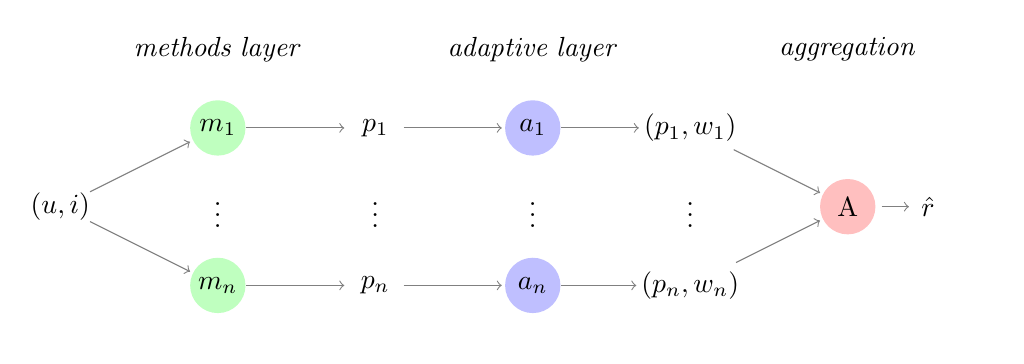
\begin{tikzpicture}[shorten >=1pt,->,draw=black!50, node distance=\layersep]

    \tikzstyle{every pin edge}=[<-,shorten <=2pt]
    \tikzstyle{node}=[circle,fill=black!25,minimum size=20pt,inner sep=0pt]
    \tikzstyle{input node}=[node, fill=green!25];
    \tikzstyle{output node}=[node, fill=red!25];
    \tikzstyle{hidden node}=[node, fill=blue!25];
    \tikzstyle{annot} = [text width=10em, text centered]
    \tikzstyle{txt}=[node,fill=white];
    
    \node[txt] (UI) at (0,-2) {$(u,i)$};  

    \node[input node] (I-1) at (\layersep,-1) {$m_1$};
    \node[txt]        (I-D) at (\layersep,-2) {$\vdots$};
    \node[input node] (I-N) at (\layersep,-3) {$m_n$};
    
    \node[txt] (P-1) at (\layersep*2, -1) {$p_1$};
    \node[txt] (P-D) at (\layersep*2, -2) {$\vdots$};
    \node[txt] (P-N) at (\layersep*2, -3) {$p_n$};

    \node[hidden node] (H-1) at (\layersep*3, -1) {$a_1$};    
    \node[txt]         (H-D) at (\layersep*3, -2) {$\vdots$};    
    \node[hidden node] (H-N) at (\layersep*3, -3) {$a_n$};    

    \node[txt] (R-1) at (\layersep*4, -1) {$(p_1,w_1)$};
    \node[txt] (R-D) at (\layersep*4, -2) {$\vdots$};
    \node[txt] (R-N) at (\layersep*4, -3) {$(p_n,w_n)$};
    
    % hidden helper node
    \node[txt] (HH)  at (\layersep*5,-1) {};

    % Draw the output layer node
    \node[output node,pin={[pin edge={->}]right:$\hat{r}$}] at (\layersep*5,-2) (O) {A};
    
    \path (UI) edge (I-1);
    \path (UI) edge (I-N);

    \path (I-1) edge (P-1);
    \path (I-N) edge (P-N);

    \path (P-1) edge (H-1);
    \path (P-N) edge (H-N);

    \path (H-1) edge (R-1);
    \path (H-N) edge (R-N);

    \path (R-1) edge (O);
    \path (R-N) edge (O);

    % Annotate the layers
    \node[annot,above of=I-1, node distance=1cm] {\emph{methods layer}};
    \node[annot,above of=H-1, node distance=1cm] {\emph{adaptive layer}};
    \node[annot,above of=HH,  node distance=1cm] {\emph{aggregation}};
  \end{tikzpicture}

  \vspace{1em}
  \caption[Stacked User Modeling]{
    Stacked user modeling:
    The method layer consists of ordinary modeling methods,
    each predicting the rating between a user and an item.
    This produces a set of predicted ratings ($p$).
    The adaptive layer estimates how well each modeling method
    will perform for the current user and item,
    and weighs the predictions accordingly.
    This produces a set of predictions and weights [$(p,w)$].
    The aggregation weighs the predictions into a final score $\hat{r}$.  
  }
  \label{fig:stackedusermodeling}
\end{figure}


While they may look similar, level 2 is not the same as the method aggregation approaches we have seen in Section \ref{sec:aggregate}.
Standard aggregation methods simply combine multiple predictions into one scalar score, regardless of the current item and user.
However, in our approach, this layer are a set of fully fledged modeling method in itself, not a simple function or a set of generalized weights.
In addition, we train a separate adaptive function for each method in level 1.
By using a complete modeling method, adaptive aggregation can be achieved, as we shall soon see.

Another way of describing (and implementing) the two modeling levels is through application
of the $\mathrm{map}$ and $\mathrm{reduce}$ functions of functional programming.
When performing \emph{prediction aggregation} (scores), this estimation can be expressed as

\begin{equation*}
  \hat{r}_{ui} = \mathrm{reduce}(u, \mathrm{map}(M,u,i)).
\end{equation*}

First, each modeling method is applied through the $\mathrm{map}$ function, with the current user and rating for which
a rating should be estimated. This produces a set of scalar prediction values. These values are then
combined through the $\mathrm{reduce}$ method, which takes the predictions and current user as input.
In our case, this is the adaptive aggregation method. 
If we wish to do rank aggregation (i.e. sorted lists), the equation is a bit different:

\begin{equation*}
  \tau_{u,n} = \mathrm{reduce}(u, \mathrm{map}(M,u,n)).
\end{equation*}

Here, $\tau_{u}$ is the list of recommended items for user $u$ (following the notation in \citet[p3]{Dwork2001}).
Note that there is no input item in this formula as we wish to produce a ranking of the top $n$ recommended items.

Expressing ourselves in terms of $\mathrm{map}$ and $\mathrm{reduce}$ now is helpful, as this will later
guide our implementation of these operations in a proper MapReduce framework
for parallell computation (as explained in \citet[p75]{Manning2008}).
The $\mathrm{map}$ function may apply each modeling method in parallell, 
as these are independent computations.
The modified $\mathrm{reduce}$ function, which takes the resulting predictions $\mathrm{map}$ and the current
user as inputs, serve as our adaptive aggregator.
Let us now describe how to make this function.


\subsection{Adaptive Aggregation}

To perform adaptive aggregation, we need the $Adapters$ to be actual user modeling methods,
that adapts the blending with respect to each user and item.
Until now we have talked about both prediction aggregation (scores) and rank aggregation (sorted lists).
For now we shall stick to scalar predictions, but will return to rank aggregation in Section \ref{sec:methods:rank}.

The simplest generalized way of prediction aggregation is a simple avereage over all predictions made
by the different methods (e.g. \citet[p3]{Aslam2001}):

\begin{equation*}
  \hat{r}_{ui} = \frac{1}{N} \sum_{m \in M} p(m,u,i).
\end{equation*}

$\hat{r}_{ui}$ is the estimated rating from user $u$ to item $i$,
$N$ is the number of methods in $M$, and $p(m,u,i)$ is the predicted rating from method $m$.
However, in most cases we wish to weight each method differently (e.g. \cite{Claypool1999} ):

\begin{equation*}
  \hat{r}_{ui} = \sum_{m \in M} w_{m} \cdot p(m,u,i) 
  \quad \text{where} \quad 0 \leq w_{m} \leq 1, \quad \sum_{i \in M} (w_i) = 1.
\end{equation*}

Here, $w_m$ is the weight applied to modeling method $m$. These weights fall in the range $[0,1]$ and sum up to $1$.
As described in \ref{sec:aggregate}, these weights can be estimated using a host of machine learning methods.
The known rating data is separated into a training- and testing set, which is used to estimate optimal weights
by minimizing some error across the testing set 
(note that the training set is also split in some way into two sets to create the singular modeling methods).
However, as discussed in Section \ref{sec:reasoning},
this is still a generalized, averaged result across every user. 
The system assumes that the best average result is the best result for each individual user.

In order to leverage as many data patterns as possible, and remove the latent subjectivity,
we wish the weights to be model-, user- and item-specific. In other words,

\begin{equation*}
  \hat{r}_{ui} = \sum_{m \in M} p_{w}(m,u,i) \cdot p_{r}(m,u,i)
  \quad \text{where} \quad
  \sum_{m \in M} (p_{w}(m,u,i)) = 1.
\end{equation*}

We have reduced our mission to finding $p_{w}(m,u,i)$,
that is, predicting weights for each combination of a method, a user and an item.
How can we estimate these weights?
While we could probably estimate weights based on known ratings,
a much more straight-forward approach is to \emph{model the actual errors of a method}.
By modeling the errors of a method, we can in turn predict the error
of a method for an item and a user. 
If we know the probable errors of each prediction from a set of models,
we can weight the resulting prediction accordingly.
This will become clear later, but for now,
consider the following \emph{error matrix}:

\begin{equation*}
 E_{u,i} =
 \begin{pmatrix}
    e_{1,1} & e_{1,2} & \cdots & e_{1,i} \\
    e_{2,1} & e_{2,2} & \cdots & e_{2,i} \\
    \vdots  & \vdots  & \ddots & \vdots  \\
    e_{u,1} & e_{u,2} & \cdots & e_{u,i}
 \end{pmatrix}
\end{equation*}

Creating an error matrix for each modeling method is quite simple.
By splitting the data used to train the methods in two,
the first set can be used for the actual training, and the second
can be used to populate the error matrix.
Each method then gets an error matrix where some cells have values.
Each value corresponds to the prediction error for a combination of a user and an item.
Notice how similar this matrix is to the previously introduced ratings matrix.
This similarity is what will allow us using the exact same modeling methods
to perform adaptive aggregation.
Whenever we wish to train a new modeling method,
\emph{the modeling phase}, we apply the following algorithm:

\begin{enumerate*}
  \item Split the ratings data into two sets for training and error estimation.
  \item Train the modeling method in its specific way with the first training set.
  \item Use the error estimation data set to create the error matrix.
  \item Train a meta modeling method (error model) based on the error matrix.
\end{enumerate*}

When we have an error model for each modeling method, 
we can use these errors to estimate each weight.
Whenever we wish to create an adaptive aggregate prediction,
\emph{the prediction phase},
we apply the following algorithm:

\begin{enumerate*}
  \item Collect predictions from each modeling method for $(u,i)$.
  \item Collect estimated errors for each method for $(u,i)$.
  \item Normalize the errors so that the error vector sums to $1$.
  \item Compute a weighted combination where each weight is $1 - e_m$.
\end{enumerate*}

The next section will explain these steps in detail.
For now, we have our approach to stacked user modeling:

\begin{equation*}
  \hat{r}_{ui} = \sum_{(m_{e}, m_{r}) \in M} (1 - p(m_{e},u,i)) \cdot p(m_{r},u,i),
\end{equation*}

where $p$ returns a prediction from a model for a specific user and item,
$m_{r}$ is a standard modeling method, 
and $m_{e}$ is its corresponding error modeling method.
For this equation to work as expected, the weights must be normalized:

\begin{equation*}
  0 \leq p_{e}(m,u,i) \leq 1 \quad \text{and} \quad \sum_{m \in M} (p_{e}(m,u,i)) = 1.
\end{equation*}

Notice that the \emph{only} difference between $p_e$ and $p_r$ is how they are created.
$p_r$ is trained with the standard ratings matrix, and $p_e$ is trained using the error matrix.
This means we can use \emph{any} standard modeling method to perform adaptive aggregation.
Hence, the name \emph{stacked user modeling}. Each modeling method
is stacked under another modeling method.
The result is predictions that not only consider the current user and item,
but also consider how each method will perform in each circumstance.
We will now see how this approach can be used in practice:
First we shall do prediction aggregation in a recommendation scenario,
then rank aggregation in an information retrieval scenario.

